% Standalone annotated figure for R2.1 (end-platen + blade rationale)
%  (a) Full HCA specimen with TOP wedge-marker location
%  (b) Element detail with f^t_{pw_n} (normal) + f^t_{pw_t} (tangential)
%      contact-force arrows at one representative particle--top-platen
%      contact (notation matches Appendix A, Table 3).
%
% Compile: pdflatex fig_r2_1_platen.tex

\documentclass[border=5pt,tikz]{standalone}
\usepackage{tikz}
\usepackage{graphicx}
\usepackage{amsmath,amssymb}
\usetikzlibrary{positioning, calc, arrows.meta}

\begin{document}

\begin{tikzpicture}[
    every node/.style={font=\small},
]

%% ── Image widths (cm) ──
\def\Wfull{6.0}
\def\Wdet{6.0}
\def\gap{0.5}

%% ── (a) Full HCA with top-marker ──
\node[anchor=south west, inner sep=0] (full) at (0,0)
  {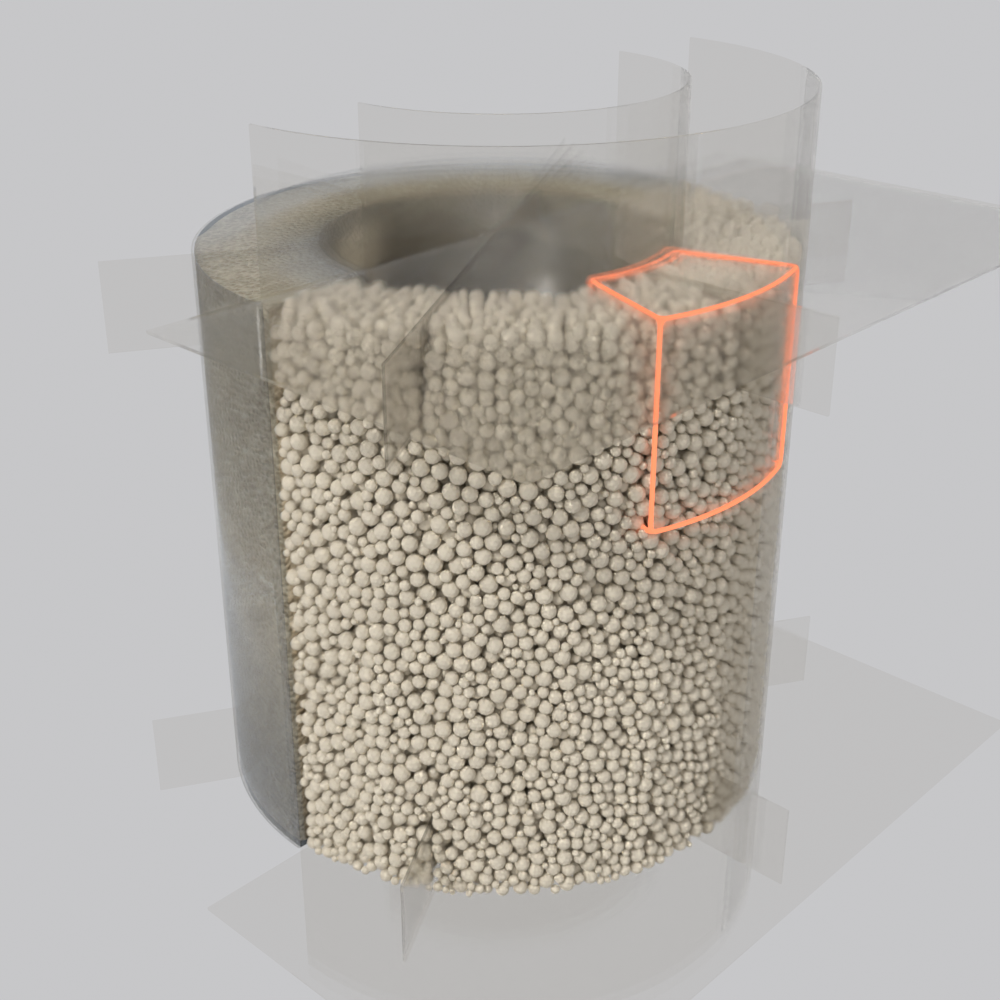
\includegraphics[width=\Wfull cm]{../rcell_full_top.png}};
\node[below=2pt of full.south] {\textbf{(a)} HCA specimen};

%% ── (b) Top-wedge detail with force arrows ──
\node[anchor=south west, inner sep=0] (det) at ({\Wfull + \gap},0)
  {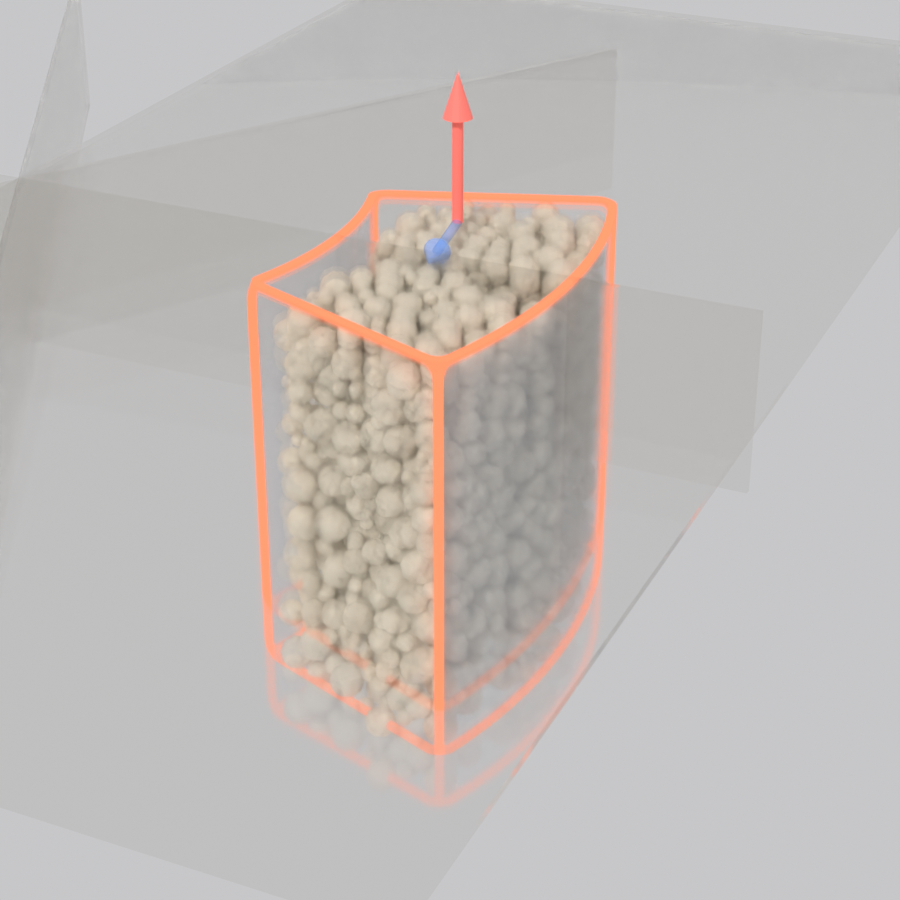
\includegraphics[width=\Wdet cm]{../rcell_detail_top_forces.png}};
\node[below=2pt of det.south] {\textbf{(b)} Particle--top-platen contact};

%% ── Connector arrow from top-marker on (a) to (b) ──
% Marker center in CamFull projection: (u,v) ≈ (0.69, 0.61) from bottom-left
\coordinate (markA)  at ($(full.south west) + (0.69*\Wfull, 0.61*\Wfull)$);
\coordinate (enterB) at ($(det.south west)  + (0.20*\Wdet,  0.61*\Wdet)$);
\draw[->, very thick, orange!75!black] (markA) -- (enterB);

%% ── Labels for force arrows on (b) ──
% Projections from CamWedgeTop (v from BOTTOM):
%   contact (tail) : (0.42, 0.66)
%   f_n head       : (0.42, 0.84)
%   f_t head       : (0.51, 0.70)
% Labels placed just beyond each head.
\node[font=\footnotesize, red!70!black] at
  ($(det.south west) + (0.58*\Wdet, 0.88*\Wdet)$)
  {$f_{pw_n}^{t}$};
\node[font=\footnotesize, blue!60!black] at
  ($(det.south west) + (0.46*\Wdet, 0.68*\Wdet)$)
  {$f_{pw_t}^{t}$};

\end{tikzpicture}

\end{document}
